\documentclass[aspectratio=169]{beamer}

\usetheme{Warsaw}
\usepackage[utf8]{inputenc}
\usepackage{tikz}
\usepackage{bm}
\usepackage{pgfplots}
\usepackage{graphicx}
\usepackage{gensymb}
\usepackage{sidecap}
\usepackage{wasysym}
\usepackage{fancybox}

%HANDOUT
%\usepackage{pgfpages}
%\pgfpagesuselayout{2 on 1}[a4paper,border shrink=5mm]
%\setbeameroption{show notes on second screen=bottom}

\pgfplotsset{compat=1.4}
\usepgfplotslibrary{units}
\usetikzlibrary{tikzmark}

\setbeamertemplate{footline}[frame number]
\setbeamertemplate{frametitle}[default][center]

\mode<presentation>{
	\usetheme{Warsaw}
	%\setbeamercovered{transparent}
	\usecolortheme{seagull}
}

\setbeamertemplate{headline}{}

\definecolor{pemblue}{RGB}{1,123,165}
\setbeamercolor*{palette primary}{fg=black,bg=pemblue!80}
\setbeamercolor*{palette secondary}{fg=black,bg=pemblue!80!gray!80}
\setbeamercolor*{palette tertiary}{fg=black,bg=pemblue!100}
\setbeamercolor*{palette quaternary}{fg=black,bg=pemblue!110}

\uselanguage{portuguese}
\languagepath{portuguese}
%\deftranslation[to=portuguese]{Definition}{Definição}
%\deftranslation[to=portuguese]{Corollary}{Identidades}

\usepackage{pgfpages}
\setbeameroption{show notes}
\setbeamertemplate{note page}[plain]
\setbeamerfont{note page}{size=\tiny}

\usebackgroundtemplate
{%
	\begin{picture}(210,40)(-5,2)
	
\includegraphics[width=0.07\paperwidth,keepaspectratio]{imgs/pem-logo-short.png}
	\end{picture}%
}

\title{Estimation of thermal contact conductance on irregular interfaces using the
	Reciprocity Functional approach}
\author{Guilherme C. de Freitas, Marcelo J. Colaço}
\date{August 16, 2021}

\institute
{
	Universidade Federal do Rio de Janeiro\\
	UFRJ/COPPE/PEM
}


\newcommand{\graficostemperatura}[5]{%
	\begin{minipage}[t][6cm][c]{4.5cm}
		\centering		
		\begin{tikzpicture}[scale=0.75]
		\begin{axis}[
		%/pgf/number format/1000 sep={.},/pgf/number format/use comma,
		axis lines=left,
		%		xmin = 0,
		%		xmax = 0.04,
		%ymin = #4,
		%ymax = #5,
		%		restrict y to domain=-500:2000,
		scaled x ticks = false,
		scaled y ticks = false,
		x tick label style={/pgf/number format/fixed},
		y tick label style={/pgf/number format/fixed},
		anchor=east,  
		width=7cm,
		height=5cm,
		label style={font=\footnotesize},
		xlabel = $x$(m),
		ylabel= $T_1\big|_{\Gamma_0}$ (\celsius),
		ylabel style={rotate=-90, at={(-0.1, 1)}, anchor = south west}]		
		\pgfplotstableread{../data/temperaturas_sinteticas_interface_0#1_conductance_0#2_stdev_05.dat} 
		\teff
		\addplot[only marks,color=gray,mark=triangle,mark options={mark size=2.0pt}] table from \teff;
		\pgfplotstableread{../data/temperaturas_sinteticas_interface_0#1_conductance_0#2_stdev_01.dat} 
		\teff
		\addplot[only marks,color=red,mark=square,mark options={mark size=2.0pt}] table from \teff;
		\pgfplotstableread{../data/temperaturas_sinteticas_interface_0#1_conductance_0#2_stdev_00.dat} 
		\teff
		\addplot[color=blue,mark=o,mark options={mark size=2.0pt}] table from \teff;		
		\end{axis}
		\end{tikzpicture}
		\caption*{(#3) Perfil #2}
	\end{minipage}
}%

% Parametros:
% erro_rms
% delta_temperatura ou fluxo_calor
% interface_id: 1, 2, ou 3
% condutance_id: 1, 2, ou 3
% axis text
% a, b, ou c
\newcommand{\graficoerrorms}[6]{%
	\begin{minipage}[t][6cm][c]{4.5cm}
		\centering		
		\begin{tikzpicture}[scale=0.75]
		\begin{axis}[
		axis lines=left,
		%/pgf/number format/1000 sep={.},/pgf/number format/use comma,
		%ymode = log,
		grid=major,
		legend style={legend pos=north west}
		% xmin = 0.00000001,
		%		xmax = 0.04,
		%ymin = 0,
		%ymax = 90,
		scaled x ticks = true,
		scaled y ticks = true,
		x tick label style={/pgf/number format/fixed},
		y tick label style={/pgf/number format/fixed},
		xtick = {0,5,10,15,20,25,30,35,40,45,50},
		anchor=east,  
		width=7cm,
		height=6cm,
		label style={font=\footnotesize},
		xlabel = $N_j$,
		ylabel= $\log\left(\delta_{#5}\right)$,
		ylabel style={rotate=-90, at={(-0.1, 1)}, anchor = south west}]
		\pgfplotstableread{../data/#1_#2_interface_0#3_conductance_0#4_stdev_00.dat} 
		\teff
		\addplot[color=blue,mark=o,mark options={mark size=2.0pt}] table from \teff;
		\pgfplotstableread{../data/#1_#2_interface_0#3_conductance_0#4_stdev_01.dat} 
		\teff
		\addplot[color=red,mark=square,mark options={mark size=2.0pt}] table from \teff;
		\pgfplotstableread{../data/#1_#2_interface_0#3_conductance_0#4_stdev_05.dat} 
		\teff
		\addplot[color=gray,mark=triangle,mark options={mark size=2.0pt}] table from \teff;
		\end{axis}
		\end{tikzpicture}
		\caption*{(#6)Perfil #4}
	\end{minipage}
}%

%Parametros
% delta_temperatura ou fluxo_calor
% interface_idx : 1, 2, ou 3
% condutance_idx : 1, 2, ou 3
% numero de autofunces para cada desvio padrao, com dois algarismos
% a, b, ou c
\newcommand{\graficoestimativa}[9]{%
	\begin{minipage}[c][3cm][c]{0.3\textwidth}
		\centering		
		\begin{tikzpicture}[scale=0.65]
		\begin{axis}[
		axis lines=left,
		%/pgf/number format/1000 sep={.},/pgf/number format/use comma,
		%		xmin = 0,
		%		xmax = 0.04,
		%		ymin = 310,
		%		ymax = 340,
		%		restrict y to domain=-500:2000,
		scaled x ticks = false,
		scaled y ticks = false,
		x tick label style={/pgf/number format/fixed},
		y tick label style={/pgf/number format/fixed},
		anchor=east,  
		width=5cm,
		height=4cm,
		label style={font=\footnotesize},
		xlabel = $x$(m),
		ylabel= $#8$ (#9),
		ylabel style={rotate=-90, at={(-0.1, 1)}, anchor = south west}]
		\pgfplotstableread{../data/comsol/#1_interface_0#2_conductance_0#3.dat} 
		\teff
		\addplot[color=black, line width=1.5pt] table from \teff;
		\pgfplotstableread{../data/fortran/#1_interface_0#2_conductance_0#3_stdev_00_N_#4.dat} 
		\teff
		\addplot[only marks, color=blue,mark=o,mark options={mark size=1.5pt}] table from \teff;
		\pgfplotstableread{../data/fortran/#1_interface_0#2_conductance_0#3_stdev_01_N_#5.dat} 
		\teff
		\addplot[only marks,color=red,mark=square,mark options={mark size=1.5pt}] table from \teff;
		\pgfplotstableread{../data/fortran/#1_interface_0#2_conductance_0#3_stdev_05_N_#6.dat} 
		\teff
		\addplot[only marks,color=gray,mark=triangle,mark options={mark size=1.5pt}] table from \teff;
		\end{axis}
		\end{tikzpicture}
		%\caption*{(#7) Perfil #3}
	\end{minipage}
}%

\newcommand{\graficoctc}[4]{%
	\begin{minipage}[t][3cm][c]{0.3\textwidth}
		\centering		
		\begin{tikzpicture}[scale=0.65]
		\begin{axis}[
		axis lines=left,
		%/pgf/number format/1000 sep={.},/pgf/number format/use comma,
		%		xmin = 0,
		%		xmax = 0.04,
		%		ymin = 310,
		%		ymax = 340,
		%		restrict y to domain=-500:2000,
		scaled x ticks = false,
		scaled y ticks = false,
		x tick label style={/pgf/number format/fixed},
		y tick label style={/pgf/number format/fixed},
		anchor=east,  
		width=5cm,
		height=4cm,
		label style={font=\footnotesize},
		xlabel = $x$(m),
		ylabel= $h_c$ (W/$\text{m}^2$\celsius),
		ylabel style={rotate=-90, at={(-0.1, 1)}, anchor = south west}]
		\pgfplotstableread{../data/conductance_#2.dat} 
		\teff
		\addplot[color=black, line width=1.5pt] table from \teff;
		\pgfplotstableread{../data/estimativa_ctc_interface_#1_conductance_#2_stdev_00.dat} 
		\teff
		\addplot[only marks, color=blue,mark=o,mark options={mark size=1.5pt}] table from \teff;
		\pgfplotstableread{../data/estimativa_ctc_interface_#1_conductance_#2_stdev_01.dat} 
		\teff
		\addplot[only marks,color=red,mark=square,mark options={mark size=1.5pt}] table from \teff;
		\pgfplotstableread{../data/estimativa_ctc_interface_#1_conductance_#2_stdev_05.dat} 
		\teff
		\addplot[only marks,color=gray,mark=triangle,mark options={mark size=1.5pt}] table from \teff;
		\end{axis}
		\end{tikzpicture}
		%\caption*{(#4) Perfil #3}
	\end{minipage}
}%

\newcommand{\graficosmetricas}[4]{%
	\begin{minipage}[t][6cm][c]{4.5cm}
	\centering		
	\begin{tikzpicture}[scale=0.75]
	\begin{axis}[
	%/pgf/number format/1000 sep={.},/pgf/number format/use comma,
	axis lines=left,
	ymode = log,
	scaled x ticks = false,
	scaled y ticks = false,
	x tick label style={/pgf/number format/fixed},
	y tick label style={/pgf/number format/fixed},
	anchor=east,  
	width=7cm,
	height=5cm,
	label style={font=\footnotesize},
	xlabel = $x$(m),
	ylabel= $T_1\big|_{\Gamma_0}$ (\celsius),
	ylabel style={rotate=-90, at={(-0.1, 1)}, anchor = south west}]			
	\addplot[color=blue,mark=triangle,mark options={mark size=2.0pt}] table[x index=0,y index=#4] {../data/erro_rms_interface_0#1_conductance_0#2_stdev_0#3.dat};				
	\end{axis}
	\end{tikzpicture}
	%\caption*{(#3) Perfil #2}
	\end{minipage}
}%

\newcommand{\graficointerface}[1]{%
	\begin{minipage}[c][2cm][c]{\textwidth}
	\centering
	\begin{tikzpicture}[scale=0.5]
	\begin{axis}[
	anchor=east,  
	ticks=none,
	width=6cm,
	height=3cm,
	%ylabel=Iterações Lineares,
	xmin = 0,
	xmax = 0.04,
	ymin = 0,
	ymax = 0.02]
	\pgfplotstableread{../data/interface_0#1.dat} 
	\teff
	\addplot[color=blue,mark=none,smooth] table from \teff;
	\end{axis}			
	\end{tikzpicture}	
	\end{minipage}
}%

\newcommand{\graficosctclegenda}{%
	\begin{minipage}[c][2cm][c]{0.3\textwidth}
	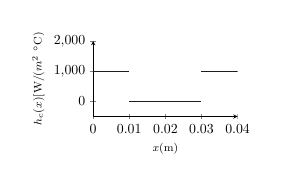
\begin{tikzpicture}[scale=0.5]
	\begin{axis}[
	%/pgf/number format/1000 sep={.},/pgf/number format/use comma,
	axis lines=left,
	xmin = 0,
	xmax = 0.04,
	ymin = -500,
	ymax = 2000,
	restrict y to domain=-500:2000,
	scaled x ticks = false,
	scaled y ticks = false,
	x tick label style={/pgf/number format/fixed},
	y tick label style={/pgf/number format/fixed},
	anchor=east,  
	width=5.25cm,
	height=3.5cm,
	label style={font=\footnotesize},
	xlabel = $x$(m),
	ylabel= $h_c(x)[$W/($\text{m}^2$ \celsius)]]
	\addplot[color=blue,mark=none,smooth, domain=0:0.01] {1000};
	\addplot[color=blue,mark=none,smooth, domain=0.01:0.03] {0};
	\addplot[color=blue,mark=none,smooth, domain=0.03:0.04] {1000};
	\end{axis}			
	\end{tikzpicture}	
	\end{minipage}
	\begin{minipage}[c][2cm][c]{0.3\textwidth}
	\begin{tikzpicture}[scale=0.5]
	\begin{axis}[
	%/pgf/number format/1000 sep={.},/pgf/number format/use comma,
	axis lines=left,
	xmin = 0,
	xmax = 0.04,
	ymin = -500,
	ymax = 2000,
	restrict y to domain=-500:2000,
	scaled x ticks = false,
	scaled y ticks = false,
	x tick label style={/pgf/number format/fixed},
	y tick label style={/pgf/number format/fixed},
	anchor=east,  
	width=5.25cm,
	height=3.5cm,
	label style={font=\footnotesize},
	xlabel = $x$(m),
	ylabel= $h_c(x)$[W/($\text{m}^2$ \celsius)]]
	\pgfplotstableread{../data/conductance_02.dat} 
	\teff
	\addplot[color=blue,mark=none,smooth] table from \teff;
	\end{axis}			
	\end{tikzpicture}	
	\end{minipage}
	\begin{minipage}[c][2cm][c]{0.3\textwidth}
	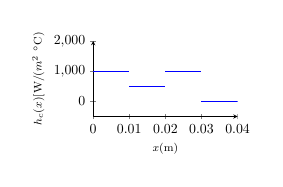
\begin{tikzpicture}[scale=0.5]
	\begin{axis}[
	%/pgf/number format/1000 sep={.},/pgf/number format/use comma,
	axis lines=left,
	xmin = 0,
	xmax = 0.04,
	ymin = -500,
	ymax = 2000,
	restrict y to domain=-500:2000,
	scaled x ticks = false,
	scaled y ticks = false,
	x tick label style={/pgf/number format/fixed},
	y tick label style={/pgf/number format/fixed},
	anchor=east,  
	width=5.25cm,
	height=3.5cm,
	label style={font=\footnotesize},
	xlabel = $x$(m),
	ylabel= $h_c(x)$[W/($\text{m}^2$ \celsius)]]
	\addplot[color=blue,mark=none,smooth, domain=0:0.01] {1000};
	\addplot[color=blue,mark=none,smooth, domain=0.01:0.02] {500};
	\addplot[color=blue,mark=none,smooth, domain=0.02:0.03] {1000};
	\addplot[color=blue,mark=none,smooth, domain=0.03:0.04] {0};
	\end{axis}	
	\end{tikzpicture}	
	\end{minipage}
}%

\newcommand{\legendagraficos}{%
	\caption{$\text{--} \rightarrow \text{Exato}$; $\textcolor{blue}{\ocircle} \rightarrow \sigma = 0.0\celsius$; $\textcolor{red}{\square} \rightarrow \sigma = 0.1\celsius$; $\textcolor{gray}{\triangle} \rightarrow \sigma = 0.5 \celsius$}	
}%


% Let's get started
\begin{document}

\setbeamertemplate{caption}{\raggedright\insertcaption\par}
	
	{
		\usebackgroundtemplate{
			\begin{picture}(210,55)(-5,0)
			
\includegraphics[height=0.14\paperwidth,keepaspectratio]{imgs/pem-logo.png}
			\end{picture}%
			\begin{picture}(210,55)(-28,2)
			
\includegraphics[height=0.14\paperwidth,keepaspectratio]{imgs/coppe-logo.pdf}
			\end{picture}
		}
		\begin{frame}
			\bigskip\bigskip\bigskip\bigskip
			\titlepage
		\end{frame}
	}
	
\section{Introduction}

\begin{frame}
	\frametitle{Introduction}
	\framesubtitle{Heat transfer through the contact interface between two bodies}
	\begin{figure}[h!b]
		\begin{center}
			\begin{tikzpicture}
			\node at (0, 0)
			{
				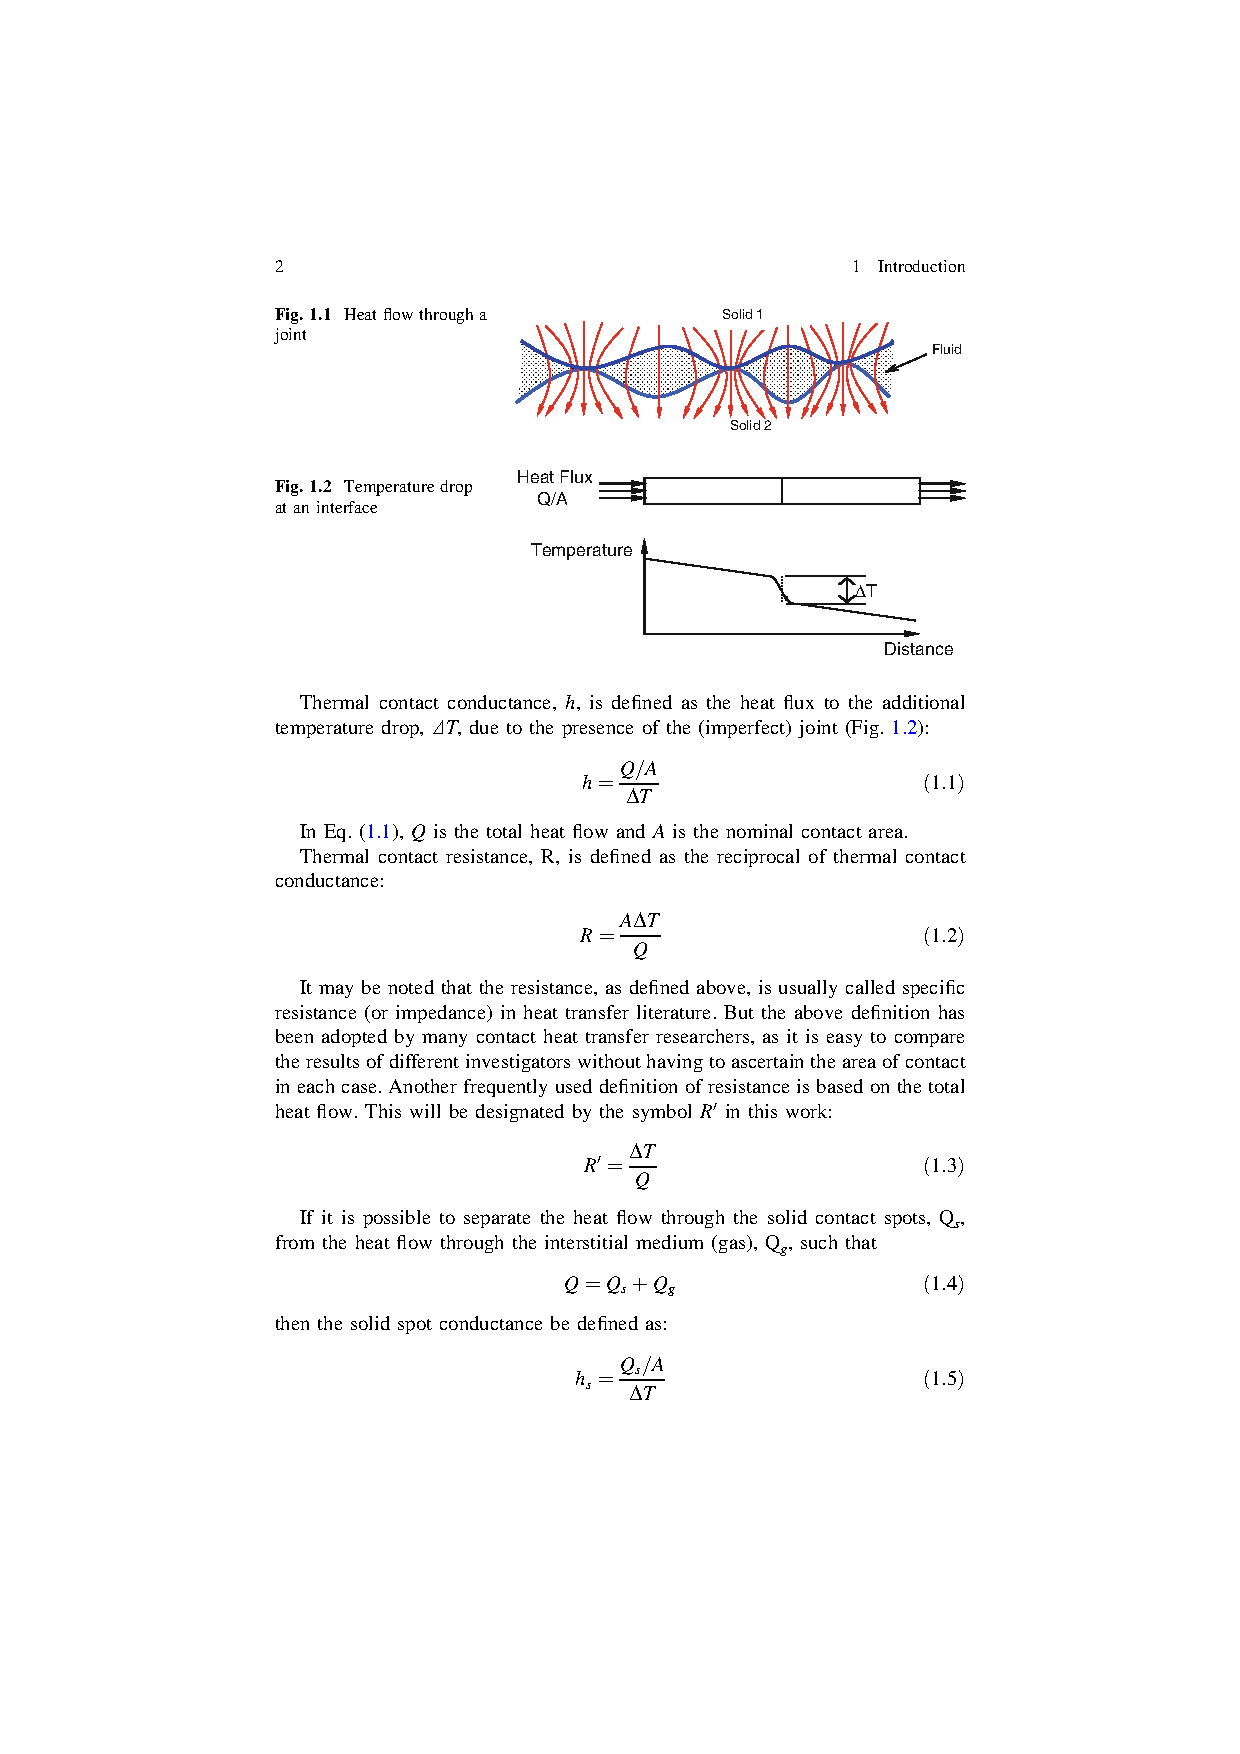
\includegraphics[trim=250 642 150 154, clip=true]{imgs/img1.pdf}
			};
			
			\node[scale=0.8] at (0, 0.9) {Soild 1};
			\node[scale=0.8] at (0, -1.1) {Solid 2};
			\node[scale=0.8] at (4, 0.3) {Fluid};
			\end{tikzpicture}
		\end{center}
	\end{figure}	
	%\note{Descrição}	
\end{frame}

\begin{frame}
	\frametitle{Introduction}
	\framesubtitle{Thermal contact conductance (TCC)}
	
	\begin{definition}{}
		\begin{equation*}
			h_c = \frac{q_c}{\Delta T_c}
		\end{equation*}
	\end{definition}
	
	\begin{alertblock}{Applications}
		\begin{itemize}
			\item Evaluating quality of contact between material bodies
			\begin{itemize}
				\item $q_c = 0 \Rightarrow h_c = 0 \Rightarrow$ perfect insulation
				\item $\Delta T_c = 0 \Rightarrow h_c = \infty \Rightarrow$ perfect contact
			\end{itemize}
			\item Identifying cracks or discontinuities in homegeneous materials
		\end{itemize}
	\end{alertblock}
\end{frame}
%
%\begin{frame}
%	\frametitle{Introdução}
%	\framesubtitle{Exemplos de áreas de aplicação}
%	\begin{itemize}
%		\item Indústria aeroespacial
%		\item Microeletrônica
%		\item Projeto de trocadores de calor
%	\end{itemize}
%\end{frame}
%
\begin{frame}
	\frametitle{Introduction}
	
	The problem of estimating TCC may be understood as an IHTP $\Rightarrow$ \textit{Inverse Heat Transfer Problem}
	
\end{frame}
%
\begin{frame}
	\frametitle{Introduction}
	\framesubtitle{Objective}
	\begin{alertblock}{}
		Study the inverse problem associated to the estimation of TCC between surfaces of two material bodies, taking into account that such surfaces are not necessarily regular.
		
		An analytical-numerical approach will be employed.
	\end{alertblock}
	\begin{center}
		%\shadowbox{COLAÇO \textit{et al.}, (2013, 2014)}
		
		%\shadowbox{COLAÇO E ALVES (2014, 2015)}
		
		\shadowbox{PADILHA \textit{et al.}, (2016)}
	\end{center}
\end{frame}
%
\begin{frame}
	\frametitle{Introduction}
	\framesubtitle{Irregular interfaces}
	\begin{figure}[h!b]
		\begin{center}
			\begin{tikzpicture}[scale=0.5]
			\begin{axis}[
			anchor=east,  
			ticks=none,
			width=8cm,
			height=4cm,
			%ylabel=Iterações Lineares,
			xmin = 0,
			xmax = 0.04,
			ymin = 0,
			ymax = 0.02]
			\pgfplotstableread{../data/interface_01.dat} 
			\teff
			\addplot[color=blue,mark=none,smooth] table from \teff;
			\end{axis}	
			\draw [very thin] (-6.4, 1.2) -- (-4.4, 2.2);
			\draw [very thin] (0.0, 1.2) -- (2.0, 2.2);
			\draw [very thin] (0.0, -1.2) -- (2.0, -0.2);
			\draw [very thin] (2.0, 2.2) -- (2.0, -0.2);
			\draw [very thin] (-4.4, 2.2) -- (2.0, 2.2);	
			\draw [very thin, blue] (0.0, -0.6) -- (2.0, 0.4);	
			\end{tikzpicture}
		\end{center}
	\end{figure}

\pause	
	
	\begin{figure}[h!b]
		\begin{center}
			\begin{tikzpicture}[scale=0.5]
			\begin{axis}[
			anchor=east,  
			ticks=none,
			width=8cm,
			height=4cm,
			%ylabel=Iterações Lineares,
			xmin = 0,
			xmax = 0.04,
			ymin = 0,
			ymax = 0.02]
			\pgfplotstableread{../data/interface_02.dat} 
			\teff
			\addplot[color=blue,mark=none,smooth] table from \teff;
			\end{axis}			
			\draw [very thin] (-6.4, 1.2) -- (-4.4, 2.2);
			\draw [very thin] (0.0, 1.2) -- (2.0, 2.2);
			\draw [very thin] (0.0, -1.2) -- (2.0, -0.2);
			\draw [very thin] (2.0, 2.2) -- (2.0, -0.2);
			\draw [very thin] (-4.4, 2.2) -- (2.0, 2.2);
			\draw [very thin, blue] (0.0, -0.6) -- (2.0, 0.4);		
			\end{tikzpicture}
		\end{center}
	\end{figure}	
\end{frame}
%
%%TODO slides de bibliografia apresentando CTC como problema inverso
%%TODO apresentar Colaço e Padilha
%%TODO apresentar CITT
%
\section{Physical problem}

\begin{frame}
	\frametitle{Physical problem}
	\framesubtitle{Physical setup}
	\begin{figure}[h!b]
		\begin{center}
			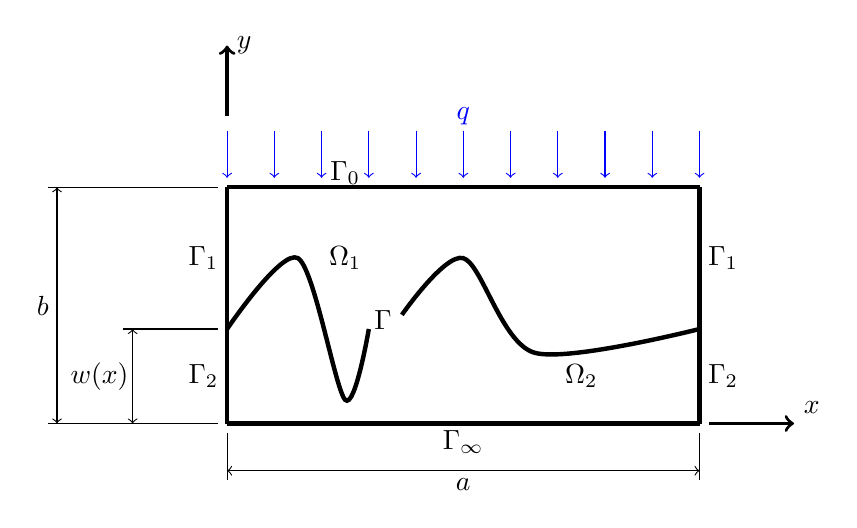
\begin{tikzpicture}[scale=0.6]
			
			\draw [ultra thick] (0, 0) -- (10, 0);
			%\draw [ultra thick] (0, 2) -- (7, 2);
			%\draw [ultra thick] (8, 2) -- (10, 2);
			\draw [ultra thick] plot [smooth] coordinates {(0, 2) (1.5, 3.5) (2.5, 0.5) (3, 2)};
			\draw [ultra thick] plot [smooth] coordinates {(3.7, 2.3) (5, 3.5) (6.5, 1.5) (10, 2)};
			\draw [ultra thick] (0, 5) -- (10, 5);
			\draw [ultra thick] (0, 0) -- (0, 5);
			\draw [ultra thick] (10, 0) -- (10, 5);
			
			\draw (2.5, 3.5) node {$\Omega_1$};
			\draw (7.5, 1) node {$\Omega_2$};	
			\draw (3.3, 2.2) node {$\Gamma$};
			\draw (-0.5, 3.5) node {$\Gamma_1$};
			\draw (-0.5, 1) node {$\Gamma_2$};
			\draw (10.5, 3.5) node {$\Gamma_1$};
			\draw (10.5, 1) node {$\Gamma_2$};
			\draw (5, -0.4) node {$\Gamma_\infty$};
			\draw (2.5, 5.3) node {$\Gamma_0$};
			\draw [blue](5, 6.5) node {$q$};
			\draw (5, -1.3) node {$a$};
			\draw (-3.9, 2.5) node {$b$};
			\draw (-2.7, 1) node {$w(x)$};
			
			\node [above right] at (12, 0) {$x$};
			\node [right] at (0, 8) {$y$};
			
			\draw [->, blue] (0, 6.2) -- (0, 5.2);
			\draw [->, blue] (1, 6.2) -- (1, 5.2);
			\draw [->, blue] (2, 6.2) -- (2, 5.2);
			\draw [->, blue] (3, 6.2) -- (3, 5.2);
			\draw [->, blue] (4, 6.2) -- (4, 5.2);
			\draw [->, blue] (5, 6.2) -- (5, 5.2);
			\draw [->, blue] (6, 6.2) -- (6, 5.2);
			\draw [->, blue] (7, 6.2) -- (7, 5.2);
			\draw [->, blue] (8, 6.2) -- (8, 5.2);
			\draw [->, blue] (9, 6.2) -- (9, 5.2);
			\draw [->, blue] (10, 6.2) -- (10, 5.2);
			
			\draw [->, very thick] (10.2,0) -- (12,0);
			\draw [->, very thick] (0, 6.5) -- (0,8);
			
			\draw [-] (0, -0.2) -- (0, -1.2);
			\draw [-] (10, -0.2) -- (10, -1.2);
			\draw [<->] (0, -1) -- (10, -1);
			
			\draw [-] (-0.2, 0) -- (-3.8, 0);
			\draw [-] (-0.2, 5) -- (-3.8, 5);
			\draw [-] (-0.2, 2) -- (-2.2, 2);
			\draw [<->] (-3.6, 0) -- (-3.6, 5);
			\draw [<->] (-2.0, 0) -- (-2.0, 2);
			
			\end{tikzpicture}
		\end{center}
	\end{figure}
	
	\begin{center}
		\shadowbox{COLAÇO and ALVES (2012); ABREU \textit{et al.} (2016)}
	\end{center}		
\end{frame}
%
\begin{frame}
	\frametitle{Physical problem}
	\framesubtitle{Formulation}
	\begin{subequations}
		\begin{alignat*}{2}
		& \nabla^2 T_1 = 0 \quad\quad\quad\quad && \text{ on } \Omega_1  \\ 
		& \nabla^2 T_2 = 0 && \text{ on }  \Omega_2\\ 
		& -k_1 \frac{\partial T_1}{\partial\mathbf{n}_1} = q && \text{ on } \Gamma_0   \\ 
		& \frac{\partial T_1}{\partial \mathbf{n}_1} = 0 && \text{ on }  \Gamma_1 \\ 
		& \frac{\partial T_2}{\partial \mathbf{n}_2} = 0 && \text{ on }  \Gamma_2 \\
		& T_2 = 0 && \text{ on }  \Gamma_\infty  \\ 
		& k_2\frac{\partial T_2}{\partial\mathbf{n}_2} = - k_1\frac{\partial T_1}{\partial\mathbf{n}_1} && \text{ on }  \Gamma \\
		& -k_1 \frac{\partial T_1}{\partial\mathbf{n}_1} = h_c(T_1-T_2) \quad\quad\quad\quad && \text{ on }  \Gamma
		\end{alignat*}
	\end{subequations}
\end{frame}
%
\section{Inverse problem}

\begin{frame}
	\frametitle{Inverse problem}
	\framesubtitle{Physical problem}
	\begin{figure}[h!b]
		\begin{center}
			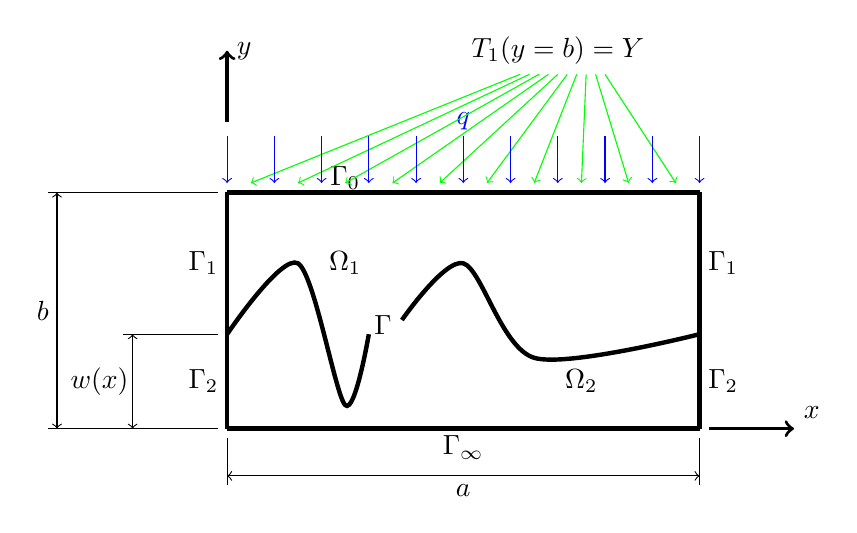
\begin{tikzpicture}[scale=0.6]
			
			\draw [ultra thick] (0, 0) -- (10, 0);
			%\draw [ultra thick] (0, 2) -- (7, 2);
			%\draw [ultra thick] (8, 2) -- (10, 2);
			\draw [ultra thick] plot [smooth] coordinates {(0, 2) (1.5, 3.5) (2.5, 0.5) (3, 2)};
			\draw [ultra thick] plot [smooth] coordinates {(3.7, 2.3) (5, 3.5) (6.5, 1.5) (10, 2)};
			\draw [ultra thick] (0, 5) -- (10, 5);
			\draw [ultra thick] (0, 0) -- (0, 5);
			\draw [ultra thick] (10, 0) -- (10, 5);
			
			\draw (2.5, 3.5) node {$\Omega_1$};
			\draw (7.5, 1) node {$\Omega_2$};	
			\draw (3.3, 2.2) node {$\Gamma$};
			\draw (-0.5, 3.5) node {$\Gamma_1$};
			\draw (-0.5, 1) node {$\Gamma_2$};
			\draw (10.5, 3.5) node {$\Gamma_1$};
			\draw (10.5, 1) node {$\Gamma_2$};
			\draw (5, -0.4) node {$\Gamma_\infty$};
			\draw (2.5, 5.3) node {$\Gamma_0$};
			\draw [blue](5, 6.5) node {$q$};
			\draw (5, -1.3) node {$a$};
			\draw (-3.9, 2.5) node {$b$};
			\draw (-2.7, 1) node {$w(x)$};
			
			\node at (7, 8) {$T_1(y=b) = Y$};
			\draw [->, green] (6.2, 7.5) -- (0.5, 5.2);
			\draw [->, green] (6.4, 7.5) -- (1.5, 5.2);
			\draw [->, green] (6.6, 7.5) -- (2.5, 5.2);
			\draw [->, green] (6.8, 7.5) -- (3.5, 5.2);
			\draw [->, green] (7, 7.5) -- (4.5, 5.2);
			\draw [->, green] (7.2, 7.5) -- (5.5, 5.2);
			\draw [->, green] (7.4, 7.5) -- (6.5, 5.2);
			\draw [->, green] (7.6, 7.5) -- (7.5, 5.2);
			\draw [->, green] (7.8, 7.5) -- (8.5, 5.2);
			\draw [->, green] (8, 7.5) -- (9.5, 5.2);
			
			\node [above right] at (12, 0) {$x$};
			\node [right] at (0, 8) {$y$};
			
			\draw [->, blue] (0, 6.2) -- (0, 5.2);
			\draw [->, blue] (1, 6.2) -- (1, 5.2);
			\draw [->, blue] (2, 6.2) -- (2, 5.2);
			\draw [->, blue] (3, 6.2) -- (3, 5.2);
			\draw [->, blue] (4, 6.2) -- (4, 5.2);
			\draw [->, blue] (5, 6.2) -- (5, 5.2);
			\draw [->, blue] (6, 6.2) -- (6, 5.2);
			\draw [->, blue] (7, 6.2) -- (7, 5.2);
			\draw [->, blue] (8, 6.2) -- (8, 5.2);
			\draw [->, blue] (9, 6.2) -- (9, 5.2);
			\draw [->, blue] (10, 6.2) -- (10, 5.2);
			
			\draw [->, very thick] (10.2,0) -- (12,0);
			\draw [->, very thick] (0, 6.5) -- (0,8);
			
			\draw [-] (0, -0.2) -- (0, -1.2);
			\draw [-] (10, -0.2) -- (10, -1.2);
			\draw [<->] (0, -1) -- (10, -1);
			
			\draw [-] (-0.2, 0) -- (-3.8, 0);
			\draw [-] (-0.2, 5) -- (-3.8, 5);
			\draw [-] (-0.2, 2) -- (-2.2, 2);
			\draw [<->] (-3.6, 0) -- (-3.6, 5);
			\draw [<->] (-2.0, 0) -- (-2.0, 2);
			
			\end{tikzpicture}
		\end{center}
	\end{figure}
\end{frame}
%
\begin{frame}
	\frametitle{Inverse problem}
	\framesubtitle{Formulation}
	\begin{alertblock}{}
	\begin{align*}
	& q_c = -k_1\frac{\partial T_1}{\partial \mathbf{n}_1}\bigg|_\Gamma
	=
	h_c[T_1 - T_2]_\Gamma \\ \\
	& \therefore h_c = \frac{-k_1\displaystyle\frac{\partial T_1}{\partial \mathbf{n}_1}\bigg|_\Gamma}{[T_1 - T_2]_\Gamma} \\
	\end{align*}
	\end{alertblock}
\end{frame}

\begin{frame}
	\frametitle{Inverse problem}
		\framesubtitle{Formulation}
		Indirect formulation of the heat flux and temperature jump across the contact interface
		
		\begin{tikzpicture}[overlay]
		\pause
		\draw (9, 0) node {\shadowbox{obtained from auxiliary problems}};			
		\draw[blue,rounded corners] (8.1, -1.3) rectangle (9.1, -1.8);
		\draw[blue,rounded corners] (8.2, -3.35) rectangle (9.2, -3.85);
		\draw [->, blue, very thick] (8.7, -0.35) -- (8.7, -1.3);
		\draw [-, blue, very thick] (9.6, -0.35) -- (9.6, -3.6);
		\draw [->, blue, very thick] (9.6, -3.6) -- (9.2, -3.6);
		\pause
		\draw (6, -5) node {\shadowbox{obtained from reciprocity functionals}};
		\draw[red,rounded corners] (7.7, -1.3) rectangle (8.1, -1.8);
		\draw[red,rounded corners] (7.9, -3.35) rectangle (8.3, -3.85);		
		\draw [->, red, very thick] (8.1, -4.65) -- (8.1, -3.85);	
		\draw [-, red, very thick] (4.3, -4.65) -- (4.3, -2.6);
		\draw [-, red, very thick] (4.3, -2.6) -- (7.9, -2.6);
		\draw [->, red, very thick] (7.9, -2.6) -- (7.9, -1.8);
		\end{tikzpicture}
		
		\begin{align*}
		& [T_1 - T_2]_\Gamma \approx \sum_{j=1}^{N_1} \alpha_j \beta_j(\Gamma) \\ \\
		& - k_1 \frac{\partial T_1}{\partial\mathbf{n_1}}\bigg|_\Gamma \approx \sum_{j=1}^{N_2} \sigma_j \gamma_j(\Gamma)
		\end{align*}
\end{frame}

\begin{frame}
	\frametitle{Inverse problem}
	\framesubtitle{Assumptions}
	\begin{itemize}
		\item \textbf{Inner product} of $f(\Gamma)$ and $g(\Gamma)$:
		\begin{align*}
		 \langle f(\Gamma), g(\Gamma) \rangle = \int_{\Gamma} f(\Gamma) g(\Gamma)d\Gamma
		\end{align*}
		\item $\beta_j(\Gamma), j=1,2,\ldots N_1$ are orthonormal, i.e:
		\begin{align*}
		\left\langle  \beta_m(\Gamma), \beta_n(\Gamma) \right\rangle = \left\lbrace
		\begin{matrix}
		0, & m \neq n \\
		1, & m = n 
		\end{matrix}
		\right.
		\end{align*}
		
		\item $\gamma_j(\Gamma), j=1,2,\ldots N_2$ are orthonormal, i.e:
		\begin{align*}
		\left\langle  \gamma_m(\Gamma), \gamma_n(\Gamma) \right\rangle = \left\lbrace
		\begin{matrix}
		0, & m \neq n \\
		1, & m = n 
		\end{matrix}
		\right.
		\end{align*}
	\end{itemize}
\end{frame}
%
\begin{frame}
	\frametitle{Inverse problem}
	\framesubtitle{Calculation of the coefficients}
	\begin{alertblock}{}
	\begin{align*}
		& \alpha_j = \left\langle [T_1 - T_2]_\Gamma, \beta_j(\Gamma) \right\rangle \\ \\
		& \sigma_j = \left\langle - k_1 \frac{\partial T_1}{\partial\mathbf{n_1}}\bigg|_\Gamma, \gamma_j(\Gamma) \right\rangle \\
	\end{align*}
\end{alertblock}
	
	These inner products will be represented in terms of measures obtained from the outer surfaces of the bodies in contact
\end{frame}
%
\section{Solution of the inverse problem (RF + CITT)}
\begin{frame}{Formulation of the auxiliary problems}
	\framesubtitle{First auxiliary problem}
	\begin{columns}
	\begin{column}{.5\textwidth}
	\begin{subequations}
		\begin{alignat*}{2}
		& \nabla^2 F_{1,j} = 0 \quad\quad\quad\quad && \text{ in } \Omega_1  \\
		& F_{1,j} = \psi_j(x) && \text{ on } \Gamma_0   \\
		& \frac{\partial F_{1,j}}{\partial \mathbf{n}_1} = 0 && \text{ on }  \Gamma_1  \\ 
		& F_{1,j} = F_{2, j} \quad\quad\quad\quad\quad && \text{ on }  \Gamma \\
		& \nabla^2 F_{2,j} = 0 && \text{ on }  \Omega_2 \\
		& \frac{\partial F_{2,j}}{\partial \mathbf{n}_2} = 0 && \text{ on }  \Gamma_2 \\
		& F_{2,j} = 0 && \text{ on }  \Gamma_\infty \\
		& k_2\frac{\partial F_{2, j}}{\partial\mathbf{n}_2} = - k_1\frac{\partial F_{1,j}}{\partial\mathbf{n}_1} && \text{ on }  \Gamma 
		\end{alignat*}
	\end{subequations}
	\end{column}
	
	\begin{column}{.5\textwidth}
		\begin{align*}
		\Rightarrow \beta_j(\Gamma) \equiv k_1 \frac{\partial F_{1,j}}{\partial\mathbf{n_1}}\bigg|_\Gamma
		\end{align*}
	\end{column}
	\end{columns}
	
	\begin{center}
		\shadowbox{ABREU (2014)}
	\end{center}
\end{frame}

\begin{frame}{Formulation of the auxiliary problems}
	\framesubtitle{Second auxiliary problem}
	\begin{columns}
	\begin{column}{.5\textwidth}
	\begin{subequations}
		\begin{alignat*}{2}
		& \nabla^2 G_{1,j} = 0 \quad\quad\quad\quad\quad && \text{ on } \Omega_1  \\ 
		& G_{1,j} = \phi_j(x) && \text{ on } \Gamma_0  \\
		& \frac{\partial G_{1,j}}{\partial \mathbf{n}_1} = 0 && \text{ on }  \Gamma_1  \\ 
		& \frac{\partial G_{1,j}}{\partial\mathbf{n}_1} = 0 \quad\quad\quad\quad\quad && \text{ on }  \Gamma 
		\end{alignat*}
	\end{subequations}
	\end{column}

	\begin{column}{.5\textwidth}
		\begin{align*}
		\Rightarrow \gamma_j(\Gamma) \equiv G_{1,j}\big|_\Gamma
	\end{align*}
	\end{column}
	\end{columns}

	\begin{center}
		\shadowbox{ABREU (2014)}
	\end{center}
\end{frame}

%
\begin{frame}
	\frametitle{Reciprocity Functional}
	\begin{definition}{}
		\begin{align*}
		\Re(F) = \int_{\Gamma_0}\left[\left(\frac{-q}{k_1}\right)F - Y\frac{\partial F}{\partial\mathbf{n_1}}\right]d\Gamma_0 \\
		\end{align*}
	\end{definition}
	
	\begin{center}
		\shadowbox{COLAÇO and ALVES (2012)}
	\end{center}
	
	\begin{center}
		\shadowbox{ANDRIEUX and BEN ABDA (1993)}
	\end{center}	
\end{frame}
%
\begin{frame}
	\label{slide_fr}
	\frametitle{Reciprocity Functionals}
	\framesubtitle{Identities}
	
	\begin{alertblock}{}
		\begin{align*}
		\int_\Gamma k_1 \frac{\partial F_{1,j}}{\partial\mathbf{n_1}}\left(T_1 - T_2\right)d\Gamma
		=
		k_1\int_{\Gamma_0}\left[\left(\frac{-q}{k_1}\right)\right. & \left.F_{1,j} - Y\frac{\partial F_{1,j}}{\partial\mathbf{n_1}}\right]d\Gamma_0
		\label{identidade_T} \\ \nonumber \\
		\int_\Gamma -k_1 G_{1,j} \frac{\partial T_1}{\partial\mathbf{n_1}}d\Gamma
		=
		k_1\int_{\Gamma_0}\left[\left(\frac{-q}{k_1}\right)\right. & \left.G_{1,j} -  Y\frac{\partial G_{1,j}}{\partial\mathbf{n_1}}\right]d\Gamma_0 \\
		\end{align*}
	\end{alertblock}
	
	\begin{center}
		\shadowbox{COLAÇO and ALVES (2012)}
	\end{center}
	
	\begin{alertblock}{}
		Relationship between \textit{temperature jump and heat flux measures across interface} $\Gamma$
		and \textit{temperature mesaures} $Y$ \textit{along surface} $\Gamma_0$
	\end{alertblock}
	\hyperlink{slide_produto_interno}{\beamergotobutton{}}
\end{frame}

\begin{frame}
	\frametitle{Reciprocity Functionals}
	\framesubtitle{Coefficients for temperature jump}
	\begin{alertblock}{}
		\begin{tikzpicture}[overlay]
		\draw[blue,rounded corners] (2.5, -0.8) rectangle (3.8, -1.9);
		\draw[blue,rounded corners] (4.95, -2.5) rectangle (5.83, -3.1);
		\draw [->, blue, thick] (3.15, -1.9) -- (5.39, -2.5);
		\end{tikzpicture}
		
		\begin{align*}
		\int_\Gamma k_1 \frac{\partial F_{1,j}}{\partial\mathbf{n_1}}\left(T_1 - T_2\right)d\Gamma		
		& =k_1\int_{\Gamma_0}\left[\left(\frac{-q}{k_1}\right)F_{1,j} - Y\frac{\partial F_{1,j}}{\partial\mathbf{n_1}}\right]d\Gamma_0
		\\ \\
		%
		\therefore \underbrace{\left\langle [T_1 - T_2]_\Gamma, \beta_j(\Gamma)\right\rangle}_{\alpha_j}
		& =
		k_1 \Re(F_{1,j}) \\
		\end{align*}		
	\end{alertblock}
\end{frame}

\begin{frame}
	\frametitle{Reciprocity Functionals}
	\framesubtitle{Coefficients for heat flux}
	\begin{alertblock}{}
		\begin{tikzpicture}[overlay]
		\draw[red,rounded corners] (3.95, -1.1) rectangle (4.6, -1.6);
		\draw[red,rounded corners] (4.6, -2.8) rectangle (5.5, -3.4);
		\draw [->, red, thick] (4.275, -1.6) -- (5.05, -2.8);
		\end{tikzpicture}
		
		\begin{align*}
		\int_\Gamma -k_1 G_{1,j} \frac{\partial T_1}{\partial\mathbf{n_1}}d\Gamma		
		& = k_1\int_{\Gamma_0}\left[\left(\frac{-q}{k_1}\right)G_{1,j} -  Y\frac{\partial G_{1,j}}{\partial\mathbf{n_1}}\right]d\Gamma_0 \\ \\
		\therefore \underbrace{\left\langle  -k_1 \frac{\partial T_1}{\partial\mathbf{n_1}}\bigg|_\Gamma, \gamma_j(\Gamma)\right\rangle}_{\sigma_j}
		& = k_1 \Re(G_{1,j})
		\\
		\end{align*}		
	\end{alertblock}
	
\end{frame}

\begin{frame}
	\frametitle{Estimates for temperature jump and heat flux across the contact interface}
	\begin{alertblock}{}
		\begin{align*}
		& [T_1 - T_2]_\Gamma = \sum_{j=1}^{N_1} k_1 \Re(F_{1,j}) \beta_j(\Gamma) \\ \\
		& - k_1 \frac{\partial T_1}{\partial\mathbf{n_1}}\bigg|_\Gamma = \sum_{j=1}^{N_2} k_1 \Re(G_{1,j}) \gamma_j(\Gamma) \\
		\end{align*}
	\end{alertblock}
\end{frame}
%
\begin{frame}
	\frametitle{Estimate for the thermal contact conductance}
	\begin{alertblock}{}
		\begin{align*}
		& h_c(x) % = \frac{- k_1 \displaystyle\frac{\partial T_1}{\partial\mathbf{n_1}}\bigg|_\Gamma}{[T_1 - T_2]_\Gamma} 
		= \frac{\displaystyle\sum_{j=1}^{N_2} \Re(G_{1,j}) \gamma_j(x)}{\displaystyle\sum_{j=1}^{N_1} \Re(F_{1,j}) \beta_j(x)} \\
		\end{align*}
	\end{alertblock}
	
	%\pause
	\begin{itemize}
		\item Indirect determination of temperature jump and heat flux across the contact interface $\rightarrow$ non-intrusive technique
		%\pause
		\item Evaluation of thermal contact conductance at any point by direct substitution in equation $\rightarrow$ non-iterative technique
	\end{itemize}
\end{frame}

\begin{frame}
	\frametitle{Solution of the auxiliary problems}
	
	Steps:
	
	\begin{enumerate}[(i)]
		\item Develop the associated eigenvalue problem
		\item Develop the appropriate transform-inverse pair
		\item Apply the integral transform to the partial differential equation of the original boundary value problem
		\item Solve the system of uncoupled ordinary differential equations
		\item Apply the inversion formula to build the complete solution
	\end{enumerate}
\end{frame}
%
%\begin{frame}
%	\frametitle{Solução dos problemas auxiliares}
%	\framesubtitle{Subdomínios}
%	\begin{figure}[h!b]
%		\begin{center}
%			\begin{tikzpicture}[scale=0.6]
%			
%			\draw [ultra thick] (0, 0) -- (10, 0);
%			\draw [ultra thick] (0, 2) -- (7, 2);
%			\draw [ultra thick] (8, 2) -- (10, 2);
%			\draw [ultra thick] (0, 5) -- (10, 5);
%			\draw [ultra thick] (0, 0) -- (0, 5);
%			\draw [ultra thick] (10, 0) -- (10, 5);
%			
%			\draw (2.5, 3.5) node {$\Omega_1$};
%			\draw (2.5, 1) node {$\Omega_2$};	
%			\draw (7.5, 2) node {$\Gamma$};
%			\draw (-0.5, 3.5) node {$\Gamma_1$};
%			\draw (-0.5, 1) node {$\Gamma_2$};
%			\draw (10.5, 3.5) node {$\Gamma_1$};
%			\draw (10.5, 1) node {$\Gamma_2$};
%			\draw (5, -0.4) node {$\Gamma_\infty$};
%			\draw (2.5, 5.3) node {$\Gamma_0$};
%			\draw [blue](5, 6.5) node {$q$};
%			\draw (5, -1.3) node {$a$};
%			\draw (-3.9, 2.5) node {$b$};
%			\draw (-2.4, 1) node {$w$};
%			
%			\node [above right] at (12, 0) {$x$};
%			\node [right] at (0, 8) {$y$};
%			
%			\draw [->, blue] (0, 6.2) -- (0, 5.2);
%			\draw [->, blue] (1, 6.2) -- (1, 5.2);
%			\draw [->, blue] (2, 6.2) -- (2, 5.2);
%			\draw [->, blue] (3, 6.2) -- (3, 5.2);
%			\draw [->, blue] (4, 6.2) -- (4, 5.2);
%			\draw [->, blue] (5, 6.2) -- (5, 5.2);
%			\draw [->, blue] (6, 6.2) -- (6, 5.2);
%			\draw [->, blue] (7, 6.2) -- (7, 5.2);
%			\draw [->, blue] (8, 6.2) -- (8, 5.2);
%			\draw [->, blue] (9, 6.2) -- (9, 5.2);
%			\draw [->, blue] (10, 6.2) -- (10, 5.2);
%			
%			\draw [->, very thick] (10.2,0) -- (12,0);
%			\draw [->, very thick] (0, 6.5) -- (0,8);
%			
%			\draw [-] (0, -0.2) -- (0, -1.2);
%			\draw [-] (10, -0.2) -- (10, -1.2);
%			\draw [<->] (0, -1) -- (10, -1);
%			
%			\draw [-] (-0.2, 0) -- (-3.8, 0);
%			\draw [-] (-0.2, 5) -- (-3.8, 5);
%			\draw [-] (-0.2, 2) -- (-2.2, 2);
%			\draw [<->] (-3.6, 0) -- (-3.6, 5);
%			\draw [<->] (-2.0, 0) -- (-2.0, 2);
%			
%			\end{tikzpicture}
%		\end{center}
%	\end{figure}
%	
%	\begin{center}
%		\shadowbox{PADILHA \textit{et al.}, (2016)}
%	\end{center}		
%\end{frame}
%
%\begin{frame}
%	\frametitle{Solução dos problemas auxiliares}
%	\framesubtitle{Extensão de domínio}
%	
%	\begin{columns}
%		\begin{column}{.5\textwidth}
%			\begin{figure}[t]
%				\begin{center}
%					\begin{tikzpicture}[scale=0.4]
%					
%					\draw [ultra thick, dashed] (0, 0) -- (10, 0);
%					%\draw [ultra thick] (0, 2) -- (7, 2);
%					%\draw [ultra thick] (8, 2) -- (10, 2);
%					\draw [ultra thick] plot [smooth] coordinates {(0, 2) (1.5, 3.5) (2.5, 0.5) (3, 2)};
%					\draw [ultra thick] plot [smooth] coordinates {(3.7, 2.3) (5, 3.5) (6.5, 1.5) (10, 2)};
%					\draw [ultra thick] (0, 5) -- (10, 5);
%					\draw [ultra thick, dashed] (0, 0) -- (0, 2);	
%					\draw [ultra thick] (0, 2) -- (0, 5);	
%					\draw [ultra thick, dashed] (10, 0) -- (10, 2);
%					\draw [ultra thick] (10, 2) -- (10, 5);
%					
%					\draw (2.5, 3.5) node {$\Omega_1$};
%					\draw (3.3, 2.2) node {$\Gamma$};
%					\draw (-0.5, 3.5) node {$\Gamma_1$};
%					\draw (-0.5, 1) node {$\Gamma_2$};
%					\draw (10.5, 3.5) node {$\Gamma_1$};
%					\draw (10.5, 1) node {$\Gamma_2$};
%					\draw (5, -0.6) node {$\Gamma_\infty$};
%					\draw (2.5, 5.5) node {$\Gamma_0$};
%					\draw [blue](5, 6.5) node {$q$};
%					%\draw (5, -1.3) node {$a$};
%					%\draw (-3.9, 2.5) node {$b$};
%					%\draw (-2.7, 1) node {$w(x)$};
%					
%					\node [above right] at (12, 0) {$x$};
%					\node [right] at (0, 8) {$y$};
%					
%					\draw [->, blue] (0, 6.2) -- (0, 5.2);
%					\draw [->, blue] (1, 6.2) -- (1, 5.2);
%					\draw [->, blue] (2, 6.2) -- (2, 5.2);
%					\draw [->, blue] (3, 6.2) -- (3, 5.2);
%					\draw [->, blue] (4, 6.2) -- (4, 5.2);
%					\draw [->, blue] (5, 6.2) -- (5, 5.2);
%					\draw [->, blue] (6, 6.2) -- (6, 5.2);
%					\draw [->, blue] (7, 6.2) -- (7, 5.2);
%					\draw [->, blue] (8, 6.2) -- (8, 5.2);
%					\draw [->, blue] (9, 6.2) -- (9, 5.2);
%					\draw [->, blue] (10, 6.2) -- (10, 5.2);
%					
%					\draw [->, very thick] (10.2,0) -- (12,0);
%					\draw [->, very thick] (0, 6.5) -- (0,8);
%					
%					%\draw [-] (0, -0.2) -- (0, -1.2);
%					%\draw [-] (10, -0.2) -- (10, -1.2);
%					%\draw [<->] (0, -1) -- (10, -1);
%					
%					%\draw [-] (-0.2, 0) -- (-3.8, 0);
%					%\draw [-] (-0.2, 5) -- (-3.8, 5);
%					%\draw [-] (-0.2, 2) -- (-2.2, 2);
%					%\draw [<->] (-3.6, 0) -- (-3.6, 5);
%					%\draw [<->] (-2.0, 0) -- (-2.0, 2);
%					
%					\end{tikzpicture}
%				\end{center}
%			\end{figure}
%		\end{column}
%		
%		\begin{column}{.5\textwidth}
%			\begin{figure}[t]
%				\begin{center}
%					\begin{tikzpicture}[scale=0.4]
%					
%					\draw [ultra thick] (0, 0) -- (10, 0);
%					%\draw [ultra thick] (0, 2) -- (7, 2);
%					%\draw [ultra thick] (8, 2) -- (10, 2);
%					\draw [ultra thick] plot [smooth] coordinates {(0, 2) (1.5, 3.5) (2.5, 0.5) (3, 2)};
%					\draw [ultra thick] plot [smooth] coordinates {(3.7, 2.3) (5, 3.5) (6.5, 1.5) (10, 2)};
%					\draw [ultra thick, dashed] (0, 5) -- (10, 5);
%					\draw [ultra thick] (0, 0) -- (0, 2);	
%					\draw [ultra thick, dashed] (0, 2) -- (0, 5);	
%					\draw [ultra thick] (10, 0) -- (10, 2);
%					\draw [ultra thick, dashed] (10, 2) -- (10, 5);
%					
%					\draw (7.5, 1) node {$\Omega_2$};	
%					\draw (3.3, 2.2) node {$\Gamma$};
%					\draw (-0.5, 3.5) node {$\Gamma_1$};
%					\draw (-0.5, 1) node {$\Gamma_2$};
%					\draw (10.5, 3.5) node {$\Gamma_1$};
%					\draw (10.5, 1) node {$\Gamma_2$};
%					\draw (5, -0.6) node {$\Gamma_\infty$};
%					\draw (2.5, 5.5) node {$\Gamma_0$};
%					\draw [blue](5, 6.5) node {$q$};
%					%\draw (5, -1.3) node {$a$};
%					%\draw (-3.9, 2.5) node {$b$};
%					%\draw (-2.7, 1) node {$w(x)$};
%					
%					\node [above right] at (12, 0) {$x$};
%					\node [right] at (0, 8) {$y$};
%					
%					\draw [->, blue] (0, 6.2) -- (0, 5.2);
%					\draw [->, blue] (1, 6.2) -- (1, 5.2);
%					\draw [->, blue] (2, 6.2) -- (2, 5.2);
%					\draw [->, blue] (3, 6.2) -- (3, 5.2);
%					\draw [->, blue] (4, 6.2) -- (4, 5.2);
%					\draw [->, blue] (5, 6.2) -- (5, 5.2);
%					\draw [->, blue] (6, 6.2) -- (6, 5.2);
%					\draw [->, blue] (7, 6.2) -- (7, 5.2);
%					\draw [->, blue] (8, 6.2) -- (8, 5.2);
%					\draw [->, blue] (9, 6.2) -- (9, 5.2);
%					\draw [->, blue] (10, 6.2) -- (10, 5.2);
%					
%					\draw [->, very thick] (10.2,0) -- (12,0);
%					\draw [->, very thick] (0, 6.5) -- (0,8);
%					
%					%\draw [-] (0, -0.2) -- (0, -1.2);
%					%\draw [-] (10, -0.2) -- (10, -1.2);
%					%\draw [<->] (0, -1) -- (10, -1);
%					
%					%\draw [-] (-0.2, 0) -- (-3.8, 0);
%					%\draw [-] (-0.2, 5) -- (-3.8, 5);
%					%\draw [-] (-0.2, 2) -- (-2.2, 2);
%					%\draw [<->] (-3.6, 0) -- (-3.6, 5);
%					%\draw [<->] (-2.0, 0) -- (-2.0, 2);
%					
%					\end{tikzpicture}
%				\end{center}
%			\end{figure}
%		\end{column}
%	\end{columns}
%\end{frame}
%
\begin{frame}
	\frametitle{Solution of the auxiliary problems}
	\framesubtitle{Analytical solution of the first auxiliary problem}
	
	\begin{alertblock}{}
		\begin{align*}
		F_{1, j}(x, y) = & \frac{\mathbb{A}_{j,0}(b - y) + \bar{\psi}_{j,0}y}{ab} + \nonumber \\
		&\frac{2}{a}\sum_{m=1}^\infty\left[\mathbb{A}_{j,m}\frac{\sinh\mu_m (b - y)}{\sinh\mu_m b} + \bar{\psi}_{j, m}\frac{\sinh\mu_m y}{\sinh\mu_m b}\right]\cos\mu_m x \\ \\
		F_{2, j}(x, y) = & \mathbb{D}_{j,0}\frac{y}{ab}  + \frac{2}{a}\sum_{m=1}^\infty\mathbb{D}_{j,m}\frac{\sinh\mu_m y}{\sinh\mu_m b} \cos\mu_m x \\
		\end{align*}
	\end{alertblock}	
	
	where
	\begin{align*}
	\mu_m = \frac{m \pi}{a}
	\end{align*}
	
\end{frame}

\begin{frame}
	\frametitle{Solution of the auxiliary problems}
	\framesubtitle{Analytical solution of the second auxiliary problem}
	
	\begin{alertblock}{}
	\begin{align*}	
		G_{1, j}(x, y) = & \frac{\mathbb{E}_{j,0}(b - y) + \bar{\phi}_{j,0}y}{ab} + \nonumber \\
		&\frac{2}{a}\sum_{m=1}^\infty\left[\mathbb{E}_{j,m}\frac{\sinh\mu_m (b - y)}{\sinh\mu_m b} + \bar{\phi}_{j, m}\frac{\sinh\mu_m y}{\sinh\mu_m b}\right]\cos\mu_m x \\
		\end{align*}
	\end{alertblock}	
	
	where
	\begin{align*}
	\mu_m = \frac{m \pi}{a}
	\end{align*}
	
\end{frame}
%
\begin{frame}
	\frametitle{Solution of the auxiliary problems}
	\framesubtitle{Coefficients of the first auxiliary problem}
	\begin{align*}
	\scriptsize \begin{bmatrix}
	\bar{a}_{0,0} & \bar{b}_{0,0} & \bar{a}_{0,1} & \bar{b}_{0,1} &  \ldots & \bar{a}_{0,M} & \bar{b}_{0,M} \\
	\bar{p}_{0,0} & \bar{q}_{0,0} & \bar{p}_{0,1} & \bar{q}_{0,1} &  \ldots & \bar{p}_{0,M} & \bar{q}_{0,M} \\
	\bar{a}_{1,0} & \bar{b}_{1,0} & \bar{a}_{1,1} & \bar{b}_{1,1} &  \ldots & \bar{a}_{1,M} & \bar{b}_{1,M} \\
	\bar{p}_{1,0} & \bar{q}_{1,0} & \bar{p}_{1,1} & \bar{q}_{1,1} &  \ldots & \bar{p}_{1,M} & \bar{q}_{1,M} \\
	\bar{a}_{2,0} & \bar{b}_{2,0} & \bar{a}_{2,1} & \bar{b}_{2,1} &  \ldots & \bar{a}_{2,M} & \bar{b}_{2,M} \\
	\bar{p}_{2,0} & \bar{q}_{2,0} & \bar{p}_{2,1} & \bar{q}_{2,1} &  \ldots & \bar{p}_{2,M} & \bar{q}_{2,M} \\
	\ldots & \ldots & \ldots & \ldots & \ddots & \ldots & \ldots\\
	\bar{a}_{M,0} & \bar{b}_{M,0} & \bar{a}_{M,1} & \bar{b}_{M,1} &  \ldots & \bar{a}_{M,M} & \bar{b}_{M,M} \\
	\bar{p}_{M,0} & \bar{q}_{M,0} & \bar{p}_{M,1} & \bar{q}_{M,1} &  \ldots & \bar{p}_{M,M} & \bar{q}_{M,M}
	\end{bmatrix}
	\begin{bmatrix}
	\mathbb{A}_{0,0} & \mathbb{A}_{1,0} & \mathbb{A}_{2,0} & \ldots & \mathbb{A}_{N,0} \\
	\mathbb{D}_{0,0} & \mathbb{D}_{1,0} & \mathbb{D}_{2,0} & \ldots & \mathbb{D}_{N,0} \\
	\mathbb{A}_{0,1} & \mathbb{A}_{1,1} & \mathbb{D}_{2,1} & \ldots & \mathbb{A}_{N,1} \\
	\mathbb{D}_{0,1} & \mathbb{D}_{1,1} & \mathbb{D}_{2,1} & \ldots & \mathbb{D}_{N,1} \\
	\ldots & \ldots & \ldots & \ddots & \ldots \\
	\mathbb{A}_{0,M} & \mathbb{A}_{1,M} & \mathbb{D}_{2,M} & \ldots & \mathbb{A}_{N,M} \\
	\mathbb{D}_{0,M} & \mathbb{D}_{1,M} & \mathbb{D}_{2,M} & \ldots & \mathbb{D}_{N,M}
	\end{bmatrix}
	\end{align*}
	
	\begin{align*}
	=
	\scriptsize
	\begin{bmatrix}
	\bar{c}_{0, 0} & \bar{c}_{0, 1} &\bar{c}_{0, 2} & \ldots & \bar{c}_{0, N} \\
	\bar{r}_{0, 0} & \bar{r}_{0, 1} &\bar{r}_{0, 2} & \ldots & \bar{r}_{0, N} \\
	\bar{c}_{1, 0} & \bar{c}_{1, 1} &\bar{c}_{1, 2} & \ldots & \bar{c}_{1, N} \\
	\bar{r}_{1, 0} & \bar{r}_{1, 1} &\bar{r}_{1, 2} & \ldots & \bar{r}_{1, N} \\
	\bar{c}_{2, 0} & \bar{c}_{2, 1} &\bar{c}_{2, 2} & \ldots & \bar{c}_{2, N} \\
	\bar{r}_{2, 0} & \bar{r}_{2, 1} &\bar{r}_{2, 2} & \ldots & \bar{r}_{2, N} \\
	\ldots & \ldots & \ldots & \ddots & \ldots \\
	\bar{c}_{M, 0} & \bar{c}_{M, 1} &\bar{c}_{M, 2} & \ldots & \bar{c}_{M, N} \\
	\bar{r}_{M, 0} & \bar{r}_{M, 1} &\bar{r}_{M, 2} & \ldots & \bar{r}_{M, N}
	\end{bmatrix}
	\end{align*}
\end{frame}

\begin{frame}
	\frametitle{Solution of the auxiliary problems}
	\framesubtitle{Coefficients of the second auxiliary problem}
	
	\begin{align*}
	\begin{bmatrix}
	\bar{u}_{0,0} & \bar{u}_{0,1} & \bar{u}_{0,2} & \ldots & \bar{u}_{0,M} \\
	\bar{u}_{1,0} & \bar{u}_{1,1} & \bar{u}_{1,2} & \ldots & \bar{u}_{1,M} \\
	\bar{u}_{2,0} & \bar{u}_{2,1} & \bar{u}_{2,2} & \ldots & \bar{u}_{2,M} \\
	\ldots & \ldots & \ddots & \ldots\\
	\bar{u}_{M,0} & \bar{u}_{M,1} & \bar{u}_{M,2} & \ldots & \bar{u}_{M,M} \\
	\end{bmatrix}
	\begin{bmatrix}
	\mathbb{E}_{0,0} & \mathbb{E}_{1,0} & \mathbb{E}_{2,0} & \ldots & \mathbb{E}_{N,0} \\
	\mathbb{E}_{0,1} & \mathbb{E}_{1,1} & \mathbb{E}_{2,1} & \ldots & \mathbb{E}_{N,1} \\
	\ldots & \ldots & \ldots & \ddots & \ldots \\
	\mathbb{E}_{0,M} & \mathbb{E}_{1,M} & \mathbb{E}_{2,M} & \ldots & \mathbb{E}_{N,M}
	\end{bmatrix}
	\end{align*}
	
	\begin{align*}	
	=
	\begin{bmatrix}
	\bar{v}_{0, 0} & \bar{v}_{0, 1} &\bar{v}_{0, 2} & \ldots & \bar{v}_{0, N} \\
	\bar{v}_{1, 0} & \bar{v}_{1, 1} &\bar{v}_{1, 2} & \ldots & \bar{v}_{1, N} \\
	\bar{v}_{2, 0} & \bar{v}_{2, 1} &\bar{v}_{2, 2} & \ldots & \bar{v}_{2, N} \\
	\ldots & \ldots & \ldots & \ddots & \ldots \\
	\bar{v}_{M, 0} & \bar{v}_{M, 1} &\bar{v}_{M, 2} & \ldots & \bar{v}_{M, N}
	\end{bmatrix}
	\end{align*}
\end{frame}

\begin{frame}
	\frametitle{Solution of the auxiliary problems}
	\framesubtitle{Orthogonalization of functions $\beta_j$ e $\gamma_j$}
	
	\begin{tikzpicture}[overlay]
%		\pause
%		\draw (5, 0) node {\shadowbox{obtidos via solução de problemas auxiliares}};			
%		\draw[blue,rounded corners] (6.65, -1.3) rectangle (7.5, -1.8);
%		\draw[blue,rounded corners] (6.7, -3.35) rectangle (7.5, -3.85);
%		\draw [->, blue, very thick] (6.9, -0.35) -- (6.9, -1.3);
%		\draw [-, blue, very thick] (7.8, -0.35) -- (7.8, -3.6);
%		\draw [->, blue, very thick] (7.8, -3.6) -- (7.5, -3.6);
%		\pause
%		\draw (5, -5) node {\shadowbox{obtidos via funcional de reciprocidade}};
%		\draw[red,rounded corners] (6.2, -1.3) rectangle (6.6, -1.8);
%		\draw[red,rounded corners] (6.3, -3.35) rectangle (6.65, -3.85);		
%		\draw [->, red, very thick] (6.5, -4.65) -- (6.5, -3.85);	
%		\draw [-, red, very thick] (2.8, -4.65) -- (2.8, -2.6);
%		\draw [-, red, very thick] (2.8, -2.6) -- (6.4, -2.6);
%		\draw [->, red, very thick] (6.4, -2.6) -- (6.4, -1.8);
		\draw (7.1, -2.8) node {\shadowbox{Gram-Schmidt orthogonalization}};
		\draw [->, red, very thick] (7.0, -2.45) -- (7.0, -1.5);
		\draw [->, red, very thick] (7.0, -3.16) -- (7.0, -4.3);	
	\end{tikzpicture}
	
	\begin{align*}
	F_{1, j}(x, y) \Rightarrow \beta_j(x) \Rightarrow \hat{\beta}_j(x) \Rightarrow \hat{F}_{1, j}(x, y)
	\end{align*}
	
	\vspace{1.5cm}
	
	\begin{align*}
	G_{1, j}(x, y) \Rightarrow \gamma_j(x) \Rightarrow \hat{\gamma}_j(x) \Rightarrow \hat{G}_{1, j}(x, y)
	\end{align*}
	
	
\end{frame}

\section{Results}
\begin{frame}
	\frametitle{Parameters used in the test problems}
	\begin{table}[H]
		\centering
		\begin{tabular}{|l|l|}
			\hline
			\textbf{Parameter} & \textbf{Value}  \\ \hline
			$a$       & 0.04 m   \\ \hline
			$b$       & 0.02 m     \\ \hline
			$k_1$     & 54 W/(m \celsius)  \\ \hline
			$k_2$     & 14 W/(m \celsius) \\ \hline
			$q$       & -100,000 W/$\text{m}^2$ \\ \hline
			$h_{max}$       & 1000 W/($\text{m}^2$ \celsius) \\ \hline
			$N_{1,max}$       & 20 \\ \hline
			$N_{2,max}$       & 20 \\ \hline
		\end{tabular}		
		\label{tabela_params}
	\end{table}
\end{frame}
%
\begin{frame}
	\frametitle{Geometrias de interface de contato}
	\begin{figure}[H]
		\centering
		\begin{minipage}[c][2cm][c]{0.3\textwidth}
			\begin{tikzpicture}[scale=0.5]
				\begin{axis}[
				anchor=east,  
				ticks=none,
				width=8cm,
				height=4cm,
				%ylabel=Iterações Lineares,
				xmin = 0,
				xmax = 0.04,
				ymin = 0,
				ymax = 0.02]
				\pgfplotstableread{../data/interface_01.dat} 
				\teff
				\addplot[color=blue,mark=none,smooth] table from \teff;
				\end{axis}			
			\end{tikzpicture}	
		\end{minipage}
		\begin{minipage}[c][2cm][c]{0.5\textwidth}
			$w(x) = \frac{b}{2}$
		\end{minipage}
		\begin{minipage}[c][2cm][c]{0.3\textwidth}
			\begin{tikzpicture}[scale=0.5]
			\begin{axis}[
			anchor=east,  
			ticks=none,
			width=8cm,
			height=4cm,
			%ylabel=Iterações Lineares,
			xmin = 0,
			xmax = 0.04,
			ymin = 0,
			ymax = 0.02]
			\pgfplotstableread{../data/interface_02.dat} 
			\teff
			\addplot[color=blue,mark=none,smooth] table from \teff;
			\end{axis}			
			\end{tikzpicture}	
		\end{minipage}
		\begin{minipage}[c][2cm][c]{0.5\textwidth}
			\begin{equation*}
				w(x) = \left\lbrace\begin{array}{ll}
				\frac{19bx^2}{8a^2}-\frac{7bx}{24a}+\frac{b}{2}, & 0 \le x < \frac{a}{3} \\
				-\frac{25bx^2}{8a^2}+\frac{27bx}{8a}-\frac{b}{9}, &  \frac{a}{3} \le x < \frac{2a}{3} \\ 
				\frac{bx^2}{8a^2}-\frac{23bx}{24a}+\frac{4b}{3}, &  \frac{2a}{3} \le x \le a
				\end{array}\right.
			\end{equation*}
		\end{minipage}
		\begin{minipage}[c][2cm][c]{0.3\textwidth}
			\begin{tikzpicture}[scale=0.5]
			\begin{axis}[
			anchor=east,  
			ticks=none,
			width=8cm,
			height=4cm,
			%ylabel=Iterações Lineares,
			xmin = 0,
			xmax = 0.04,
			ymin = 0,
			ymax = 0.02]
			\pgfplotstableread{../data/interface_03.dat} 
			\teff
			\addplot[color=blue,mark=none,smooth] table from \teff;
			\end{axis}			
			\end{tikzpicture}	
		\end{minipage}
		\begin{minipage}[c][2cm][c]{0.5\textwidth}
			$ w(x) = \frac{b}{2} + \frac{1}{20} \cos\frac{4 \pi  x}{a}$
		\end{minipage}
	\end{figure}
\end{frame}

\begin{frame}
	\frametitle{Perfis teóricos de condutância térmica de contato}
	\begin{figure}[H]
		\centering
		\begin{minipage}[c][2cm][c]{0.3\textwidth}
			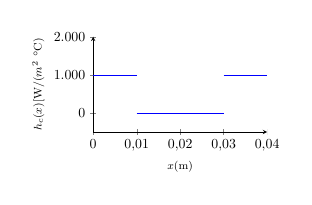
\begin{tikzpicture}[scale=0.5]
			\begin{axis}[
			/pgf/number format/1000 sep={.},/pgf/number format/use comma,
			axis lines=left,
			xmin = 0,
			xmax = 0.04,
			ymin = -500,
			ymax = 2000,
			restrict y to domain=-500:2000,
			scaled x ticks = false,
			scaled y ticks = false,
			x tick label style={/pgf/number format/fixed},
			y tick label style={/pgf/number format/fixed},
			anchor=east,  
			width=6cm,
			height=4cm,
			label style={font=\footnotesize},
			xlabel = $x$(m),
			ylabel= $h_c(x)[$W/($\text{m}^2$ \celsius)]]
			\addplot[color=blue,mark=none,smooth, domain=0:0.01] {1000};
			\addplot[color=blue,mark=none,smooth, domain=0.01:0.03] {0};
			\addplot[color=blue,mark=none,smooth, domain=0.03:0.04] {1000};
			\end{axis}			
			\end{tikzpicture}	
		\end{minipage}
		\begin{minipage}[c][2cm][c]{0.5\textwidth}
			\begin{equation*}
				h_c(x) = \left\lbrace
							\begin{array}{ll}
								h_{max}, & x < \frac{a}{4}, x > \frac{3a}{4} \\ 
								0 , & \frac{a}{4} < x < \frac{3a}{4}
							\end{array}
						\right.
			\end{equation*}
		\end{minipage}
		\begin{minipage}[c][2cm][c]{0.3\textwidth}
			\begin{tikzpicture}[scale=0.5]
			\begin{axis}[
			/pgf/number format/1000 sep={.},/pgf/number format/use comma,
			axis lines=left,
			xmin = 0,
			xmax = 0.04,
			ymin = -500,
			ymax = 2000,
			restrict y to domain=-500:2000,
			scaled x ticks = false,
			scaled y ticks = false,
			x tick label style={/pgf/number format/fixed},
			y tick label style={/pgf/number format/fixed},
			anchor=east,  
			width=6cm,
			height=4cm,
			label style={font=\footnotesize},
			xlabel = $x$(m),
			ylabel= $h_c(x)$[W/($\text{m}^2$ \celsius)]]
			\pgfplotstableread{../data/conductance_02.dat} 
			\teff
			\addplot[color=blue,mark=none,smooth] table from \teff;
			\end{axis}			
			\end{tikzpicture}	
		\end{minipage}
		\begin{minipage}[c][2cm][c]{0.5\textwidth}
			$h_c(x) = \sin\displaystyle\frac{\pi x}{a}$
		\end{minipage}
		\begin{minipage}[c][2cm][c]{0.3\textwidth}
			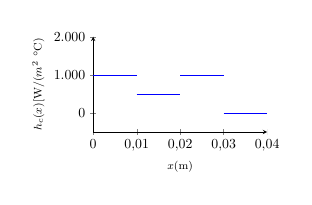
\begin{tikzpicture}[scale=0.5]
			\begin{axis}[
			/pgf/number format/1000 sep={.},/pgf/number format/use comma,
			axis lines=left,
			xmin = 0,
			xmax = 0.04,
			ymin = -500,
			ymax = 2000,
			restrict y to domain=-500:2000,
			scaled x ticks = false,
			scaled y ticks = false,
			x tick label style={/pgf/number format/fixed},
			y tick label style={/pgf/number format/fixed},
			anchor=east,  
			width=6cm,
			height=4cm,
			label style={font=\footnotesize},
			xlabel = $x$(m),
			ylabel= $h_c(x)$[W/($\text{m}^2$ \celsius)]]
			\addplot[color=blue,mark=none,smooth, domain=0:0.01] {1000};
			\addplot[color=blue,mark=none,smooth, domain=0.01:0.02] {500};
			\addplot[color=blue,mark=none,smooth, domain=0.02:0.03] {1000};
			\addplot[color=blue,mark=none,smooth, domain=0.03:0.04] {0};
			\end{axis}	
			\end{tikzpicture}	
		\end{minipage}
		\begin{minipage}[c][2cm][c]{0.5\textwidth}
			\begin{equation*}
			h_c(x) = \left\lbrace
			\begin{array}{ll}
				\displaystyle\frac{h_{max}}{2}, & x < \frac{a}{4}, \frac{a}{2} < x < \frac{3a}{4} \\
				h_{max}, & \frac{a}{4} < x < \frac{a}{2} \\
				0 , &x > \frac{3a}{4}
			\end{array}
			\right.
			\end{equation*}
		\end{minipage}
	\end{figure}
\end{frame}
%
\begin{frame}
	\frametitle{Measurement errors}
	\begin{center}
		\begin{align*}
		& \tilde{\mathbf{Y}} = \mathbf{Y} + \mathbf{\varepsilon} \sigma, \sigma = 
		\left\lbrace \begin{array}{ll}
		0.0\celsius \\
		0.1\celsius \\
		0.5\celsius
		\end{array}\right .
		\end{align*}
	\end{center}
\end{frame}

\begin{frame}
	\frametitle{Salto de temperatura, interface 1}
	\begin{figure}[H]		
		\graficointerface{1}
		\graficoestimativa{delta_temperatura}{1}{1}{20}{06}{02}{a}{\Delta T\big|_{\Gamma}}{\celsius}
		\graficoestimativa{delta_temperatura}{1}{2}{20}{04}{04}{a}{\Delta T\big|_{\Gamma}}{\celsius}
		\graficoestimativa{delta_temperatura}{1}{3}{20}{06}{03}{a}{\Delta T\big|_{\Gamma}}{\celsius}
		\legendagraficos	
		\graficosctclegenda		
	\end{figure}
\end{frame}

\begin{frame}
	\frametitle{Fluxo de calor, interface 1}
	\begin{figure}[H]		
		\graficointerface{1}
		\graficoestimativa{fluxo_calor}{1}{1}{20}{06}{04}{a}{-k_1 \frac{\partial T_1}{\partial\mathbf{n}_1}\big|_{\Gamma}}{W/$\text{m}^2$}
		\graficoestimativa{fluxo_calor}{1}{2}{20}{04}{04}{a}{-k_1 \frac{\partial T_1}{\partial\mathbf{n}_1}\big|_{\Gamma}}{W/$\text{m}^2$}
		\graficoestimativa{fluxo_calor}{1}{3}{20}{06}{04}{a}{-k_1 \frac{\partial T_1}{\partial\mathbf{n}_1}\big|_{\Gamma}}{W/$\text{m}^2$}
		\legendagraficos
		\graficosctclegenda		
	\end{figure}
\end{frame}

\begin{frame}
	\frametitle{Condutância térmica de contato, interface 1}
	\begin{figure}[H]		
		\graficointerface{1}
		\graficoctc{01}{01}{1}{a}
		\graficoctc{01}{02}{2}{b}
		\graficoctc{01}{03}{3}{c}
		\legendagraficos
		%\graficosctclegenda		
	\end{figure}
\end{frame}

\begin{frame}
	\frametitle{Salto de temperatura, interface 2}
	\begin{figure}[H]		
		\graficointerface{2}
		\graficoestimativa{delta_temperatura}{2}{1}{20}{11}{09}{a}{\Delta T\big|_{\Gamma}}{\celsius}
		\graficoestimativa{delta_temperatura}{2}{2}{20}{09}{07}{a}{\Delta T\big|_{\Gamma}}{\celsius}
		\graficoestimativa{delta_temperatura}{2}{3}{20}{11}{09}{a}{\Delta T\big|_{\Gamma}}{\celsius}
		\legendagraficos	
		\graficosctclegenda		
	\end{figure}
\end{frame}

\begin{frame}
	\frametitle{Fluxo de calor, interface 2}
	\begin{figure}[H]		
		\graficointerface{2}
		\graficoestimativa{fluxo_calor}{2}{1}{20}{10}{06}{a}{-k_1 \frac{\partial T_1}{\partial\mathbf{n}_1}\big|_{\Gamma}}{W/$\text{m}^2$}
		\graficoestimativa{fluxo_calor}{2}{2}{20}{06}{06}{a}{-k_1 \frac{\partial T_1}{\partial\mathbf{n}_1}\big|_{\Gamma}}{W/$\text{m}^2$}
		\graficoestimativa{fluxo_calor}{2}{3}{19}{09}{04}{a}{-k_1 \frac{\partial T_1}{\partial\mathbf{n}_1}\big|_{\Gamma}}{W/$\text{m}^2$}
		\legendagraficos
		\graficosctclegenda		
	\end{figure}
\end{frame}

\begin{frame}
	\frametitle{Condutância térmica de contato, interface 2}
	\begin{figure}[H]		
		\graficointerface{2}
		\graficoctc{02}{01}{1}{a}
		\graficoctc{02}{02}{2}{b}
		\graficoctc{02}{03}{3}{c}
		\legendagraficos
		%\graficosctclegenda		
	\end{figure}
\end{frame}

\begin{frame}
	\frametitle{Salto de temperatura, interface 3}
	\begin{figure}[H]		
		\graficointerface{3}
		\graficoestimativa{delta_temperatura}{3}{1}{20}{08}{06}{a}{\Delta T\big|_{\Gamma}}{\celsius}
		\graficoestimativa{delta_temperatura}{3}{2}{20}{06}{04}{a}{\Delta T\big|_{\Gamma}}{\celsius}
		\graficoestimativa{delta_temperatura}{3}{3}{20}{08}{06}{a}{\Delta T\big|_{\Gamma}}{\celsius}
		\legendagraficos	
		\graficosctclegenda		
	\end{figure}
\end{frame}

\begin{frame}
	\frametitle{Fluxo de calor, interface 3}
	\begin{figure}[H]		
		\graficointerface{3}
		\graficoestimativa{fluxo_calor}{3}{1}{20}{06}{06}{a}{-k_1 \frac{\partial T_1}{\partial\mathbf{n}_1}\big|_{\Gamma}}{W/$\text{m}^2$}
		\graficoestimativa{fluxo_calor}{3}{2}{20}{04}{04}{a}{-k_1 \frac{\partial T_1}{\partial\mathbf{n}_1}\big|_{\Gamma}}{W/$\text{m}^2$}
		\graficoestimativa{fluxo_calor}{3}{3}{20}{06}{03}{a}{-k_1 \frac{\partial T_1}{\partial\mathbf{n}_1}\big|_{\Gamma}}{W/$\text{m}^2$}
		\legendagraficos
		\graficosctclegenda		
	\end{figure}
\end{frame}

\begin{frame}
	\frametitle{Condutância térmica de contato, interface 3}
	\begin{figure}[H]		
		\graficointerface{3}
		\graficoctc{03}{01}{1}{a}
		\graficoctc{03}{02}{2}{b}
		\graficoctc{03}{03}{3}{c}
		\legendagraficos
		%\graficosctclegenda		
	\end{figure}
\end{frame}
%
\begin{frame}
	\frametitle{Stop criteria for the summations}
\begin{columns}
\begin{column}{.5\textwidth}
	\centering		
	\begin{tikzpicture}[scale=0.8]
	\begin{axis}[
	/pgf/number format/1000 sep={.},/pgf/number format/use comma,
	axis lines=left,
	ymode = log,
	scaled x ticks = false,
	scaled y ticks = false,
	x tick label style={/pgf/number format/fixed},
	y tick label style={/pgf/number format/fixed},
	anchor=east,  
	width=7cm,
	height=5cm,
	label style={font=\footnotesize},
	xlabel = $N_1$,
	ylabel= $\delta_{[T_1 - T_2]}$,
	ylabel style={rotate=-90, at={(-0.1, 1)}, anchor = south west}]			
	\addplot[only marks,color=blue,mark=o,mark options={mark size=3.0pt}] table[x index=0,y index=1] {../data/erro_rms_interface_02_conductance_01_stdev_00.dat};
	\addplot[only marks,color=red,mark=square,mark options={mark size=3.0pt}] table[x index=0,y index=1] {../data/erro_rms_interface_02_conductance_01_stdev_01.dat};
	\addplot[only marks,color=gray,mark=triangle,mark options={mark size=3.0pt}] table[x index=0,y index=1] {../data/erro_rms_interface_02_conductance_01_stdev_05.dat};			
	\end{axis}
	\end{tikzpicture}
\end{column}

\begin{column}{.5\textwidth}
	\centering		
	\begin{tikzpicture}[scale=0.8]
	\begin{axis}[
	/pgf/number format/1000 sep={.},/pgf/number format/use comma,
	axis lines=left,
	ymode = log,
	scaled x ticks = false,
	scaled y ticks = false,
	x tick label style={/pgf/number format/fixed},
	y tick label style={/pgf/number format/fixed},
	anchor=east,  
	width=7cm,
	height=5cm,
	label style={font=\footnotesize},
	xlabel = $N_2$,
	ylabel= $\delta_{\left[-k_1 \frac{\partial T_1}{\partial \mathbf{n}}\right]}$,
	ylabel style={rotate=-90, at={(-0.1, 1)}, anchor = south west}]			
	\addplot[only marks,color=blue,mark=o,mark options={mark size=3.0pt}] table[x index=0,y index=2] {../data/erro_rms_interface_02_conductance_01_stdev_00.dat};
	\addplot[only marks,color=red,mark=square,mark options={mark size=3.0pt}] table[x index=0,y index=2] {../data/erro_rms_interface_02_conductance_01_stdev_01.dat};
	\addplot[only marks,color=gray,mark=triangle,mark options={mark size=3.0pt}] table[x index=0,y index=2] {../data/erro_rms_interface_02_conductance_01_stdev_05.dat};			
	\end{axis}
	\end{tikzpicture}
\end{column}
\end{columns}
$\text{--} \rightarrow \text{Exact}$; $\textcolor{blue}{\ocircle} \rightarrow \sigma = 0.0\celsius$; $\textcolor{red}{\square} \rightarrow \sigma = 0.1\celsius$; $\textcolor{gray}{\triangle} \rightarrow \sigma = 0.5 \celsius$

%\begin{center}
%PADILHA (2006): $N_1 \le 14; N_2 \le 14$
%\end{center}

\end{frame}

%

\section{Conclusion}
\begin{frame}
	\frametitle{Conclusion}
	\begin{itemize}
		\item Direct, non-iterative method, with low computational cost, avoiding intrusive measurements inside the bodies in contact		
	\pause
		\item Calculation of very good estimates, especially for cases in which measurement noises were not added to the experimental temperature measures
	\pause
		\item Qualitative behavior of cases with measurement noises were consistent with the expected theoretical behavior
	\pause
		\item The method was able to recover the distributions of temperature jump and heat flux across the contact interface, and consequently the thermal contact conductance profile, in a fast and effective fashion
	\end{itemize}
\end{frame}

\begin{frame}
	\centering
	Thank you!
\end{frame}

	
\end{document}